%\chapter{Neuron Input/Output}
\chapter{Nerve Signals (input/output) and Intracellular signaling cascades}
\label{chap:nerve-signals}

An important part when modelling neurons' activities is the modelling of their
connections, the synapses. The mathematical model should be able to reproduce
the so-called synaptic plasticity, i.e. the change in synaptic weights $w_{ij}$.

We will consider a model neuron that is receiving multiple excitatory and
inhibitory inputs (excitatory and inhibitory postsynaptic potentials - EPSPs and
IPSPs) in the somatodendritic region that summate and bring about membrane
potential changes at the axon initial segment (AIS) - Sect.\ref{sec:AIS}.
It is in this region that voltage-gated sodium (Nav - Chap.\ref{chap:Na_models})
and certain voltage-gated potassium (Kv) channels such as the KCNQ channel
determine the threshold for firing an action potential, thereby causing action
potential generation.
Action potentials then propagate along the axon and, in the case of myelinated
axons, 'jump' between the nodes of Ranvier through saltatory conduction
to reach the nerve terminals, where activation of voltage-gated calcium (Cav)
channels causes calcium influx and neurotransmitter release.

\begin{figure}[hbt]
  \centerline{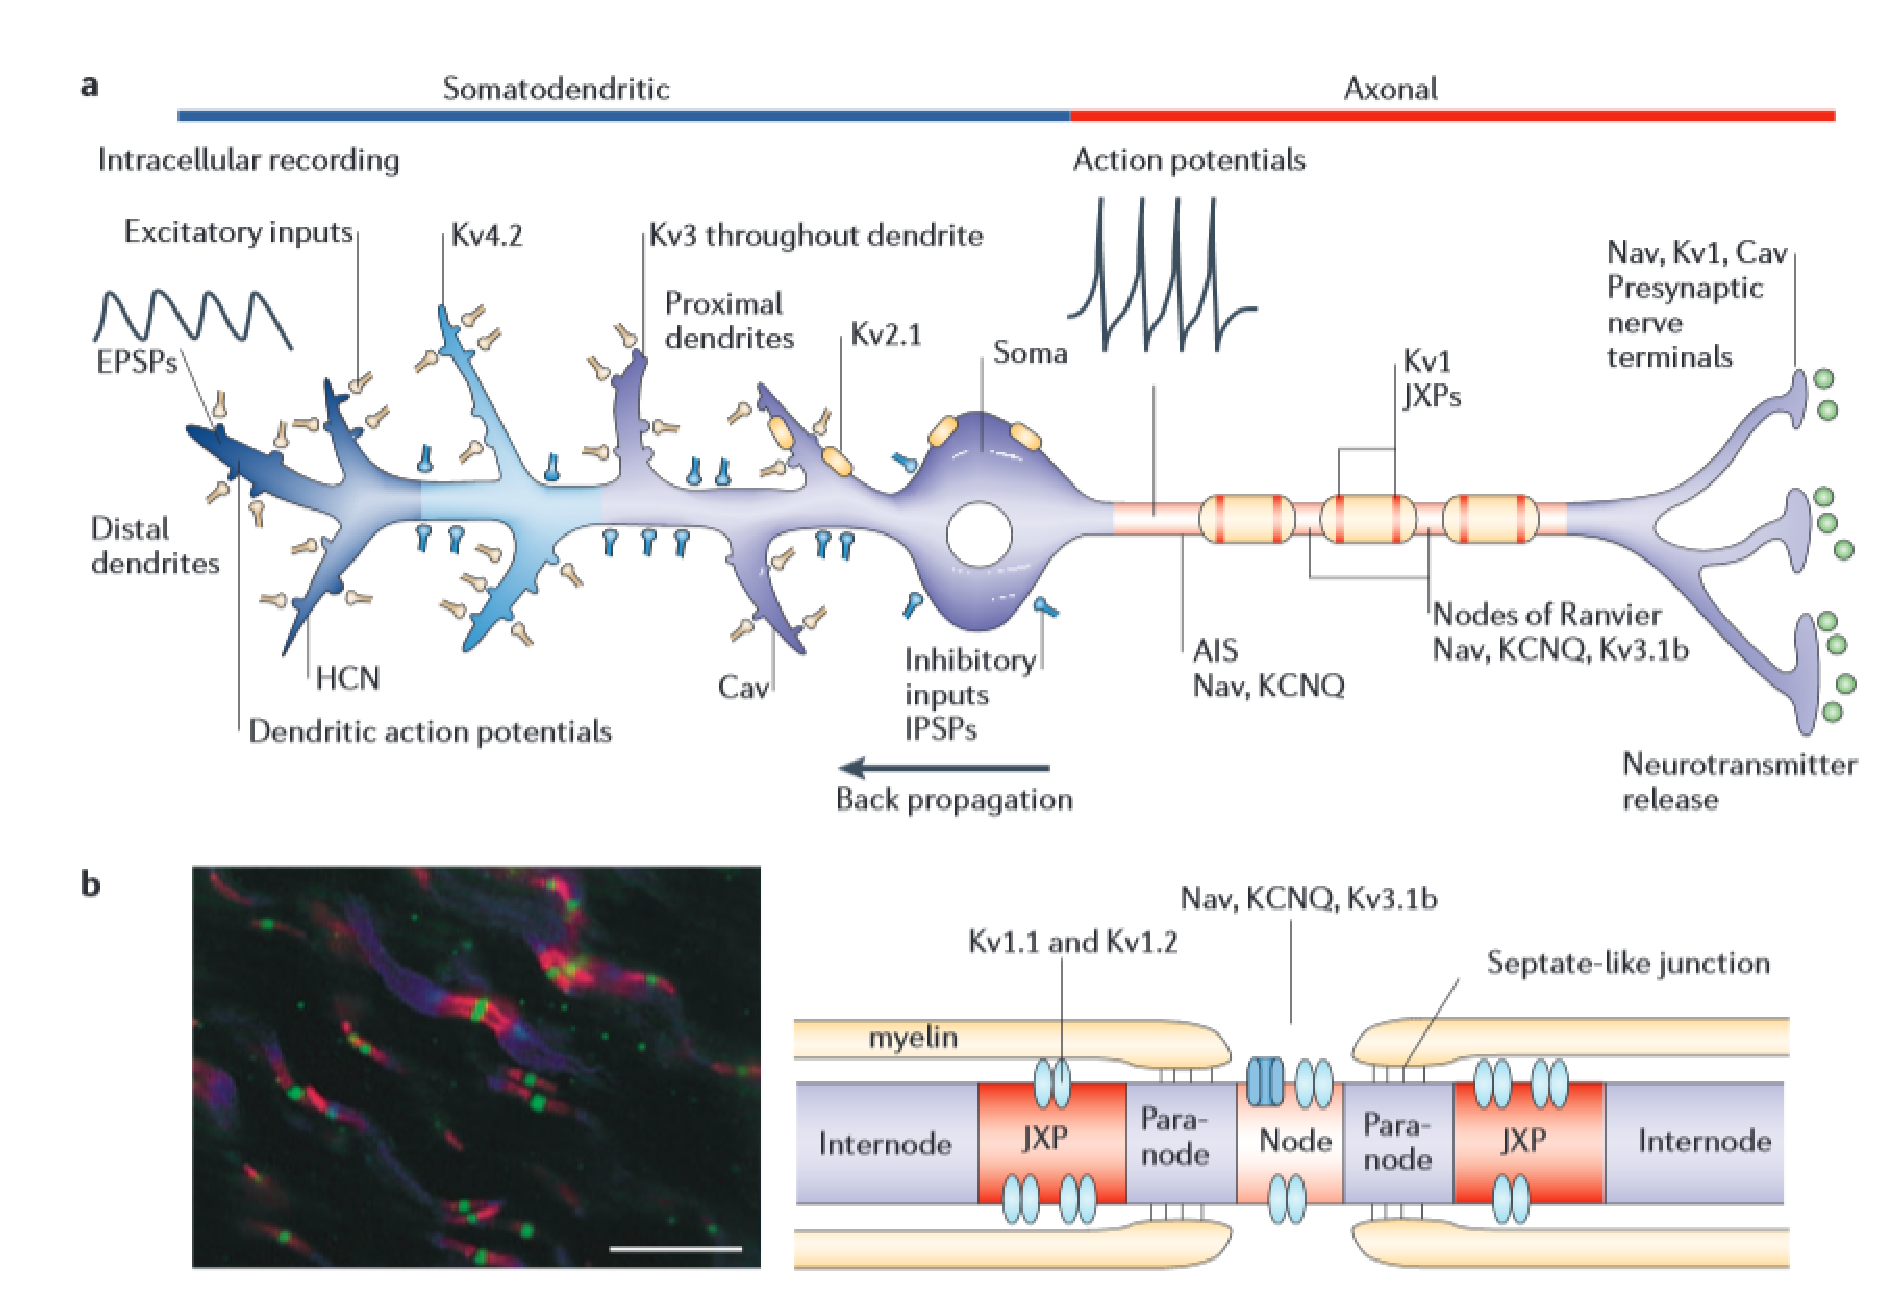
\includegraphics[height=8cm,
    angle=0]{./images/neuron-input-output.eps}}
\caption{Diagram of a neuron with inputs}
\label{fig:neuron-input-output}
\end{figure}

For pyramidal neurons, Kv channels (Sect.\ref{sec:Kv_channel}) and
hyperpolarization-activated cyclic nucleotide-gated (HCN) cation channels
(Sect.\ref{sec:HCN-channels}) on dendrites further control action potential
back-propagation, and the time course and extent of the passive spread of
synaptic potentials (Sect.\ref{sec:back-propagating_AP}).

When modeling multiple neurons, it is important to know the mechanism of signal
transduction from one neuron to another: (1) electrical synapse (electrical
charges flow directly between neurons via gap junctions), (2) chemical synapse
(the electrical signal is converted into chemical signal in the form of
neurotransmitter releases - there are different types of neurotransmitters,
which then can be interpreted differently by the various postsynaptic neurons,
depending on the chemical receptors). Chemical synapses are highly advantageous
because they can be more tightly regulated than electrical synapses.


The morphology of mitral cells (Sect.\ref{sec:mitral-cell}) was an advantage in
early studies of synaptic processing, because the soma and the primary dendrite
could be independently stimulated by appropriate positioning of stimulating
electrodes in different layers of the olfactory bulb.

\section{Connectivity between neurons}
\label{sec:neuron_connectivities}


The brain human has about 100 billion neurons ($10^{11}$). Each neuron links to 
an average 6000-10000 other neurons via synapses, i.e. giving total of
$10^{14}-10^{15}$ connections. 
\begin{itemize}
  \item in cat visual cortex: about 84\% of synapses are excitatory, and 16\%
  are inhibitory.
\end{itemize}
\url{http://centrosome.caltech.edu/courses/cns187/references/neuronal_densities.pdf}

A typical synapse joins the terminal button of an axon (called {\it
pre-synaptic}) of one nerve cell to the head of a single dendrite (called {\it
post-synaptic}) of another cell.
Between the pre-synaptic and post-synaptic there is a small gap called {\it
synaptic cleft}. \textcolor{red}{In addition to axon-dendrite connection, there
are other types of connections within a single cell: axon-to-cell, axon-to-axon,
dendrite-to-dendrite junction.}

\subsection{Electrical synapse: electrical gap junction}
\label{sec:gap-junction}
\label{sec:electrical_synapse}

\begin{figure}[htb]
  \centerline{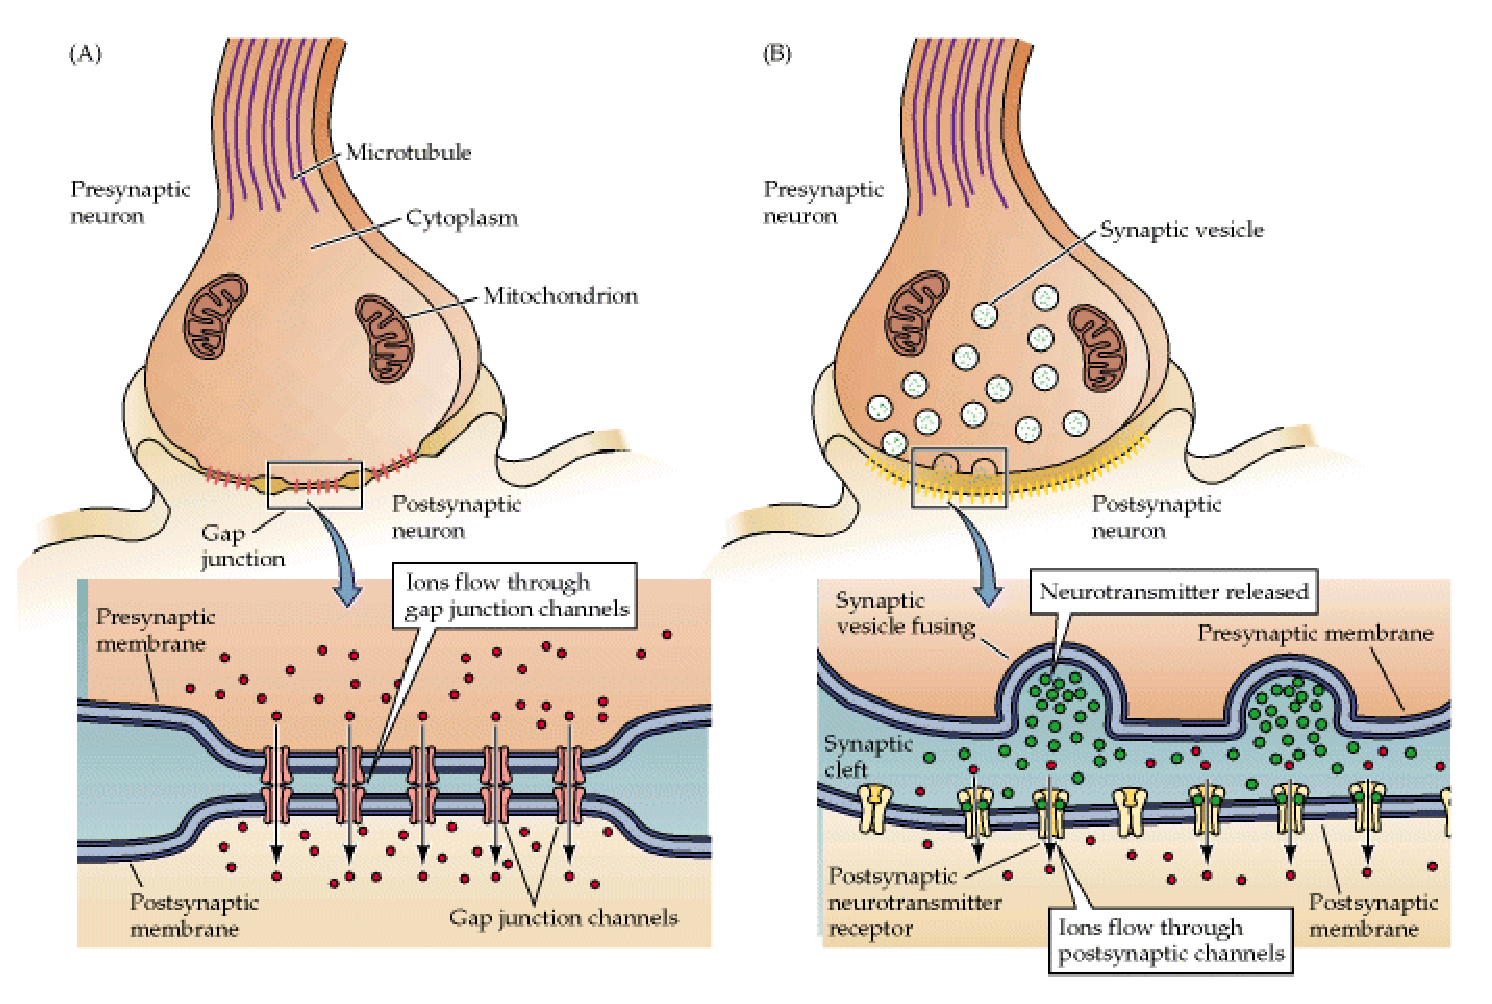
\includegraphics[height=7cm]{./images/synapse_chemical_electrical.eps}}
\caption{(A) Electrical synapse; (B) Chemical synapses}\label{fig:synapse}
\end{figure} 

The electrical synapse does not use neurotransmitter, but the electrical
current. As shown in Fig.~\ref{fig:synapse}, the gap junction in electrical
synapses contains precisely aligned, paired channels in the membrane of the
pre-synaptic and post-synaptic neurons. Each channels pair forms a pore, as
shown in Fig. \ref{fig:gap_junction}. The pore in here is much larger than the
pore in voltage-gated ion channels. This allows larger particles to be able to
transmitted from neurons to neurons, like intracellular metabolites, ATP, second
messenger.

\begin{figure}[htb]
  \centerline{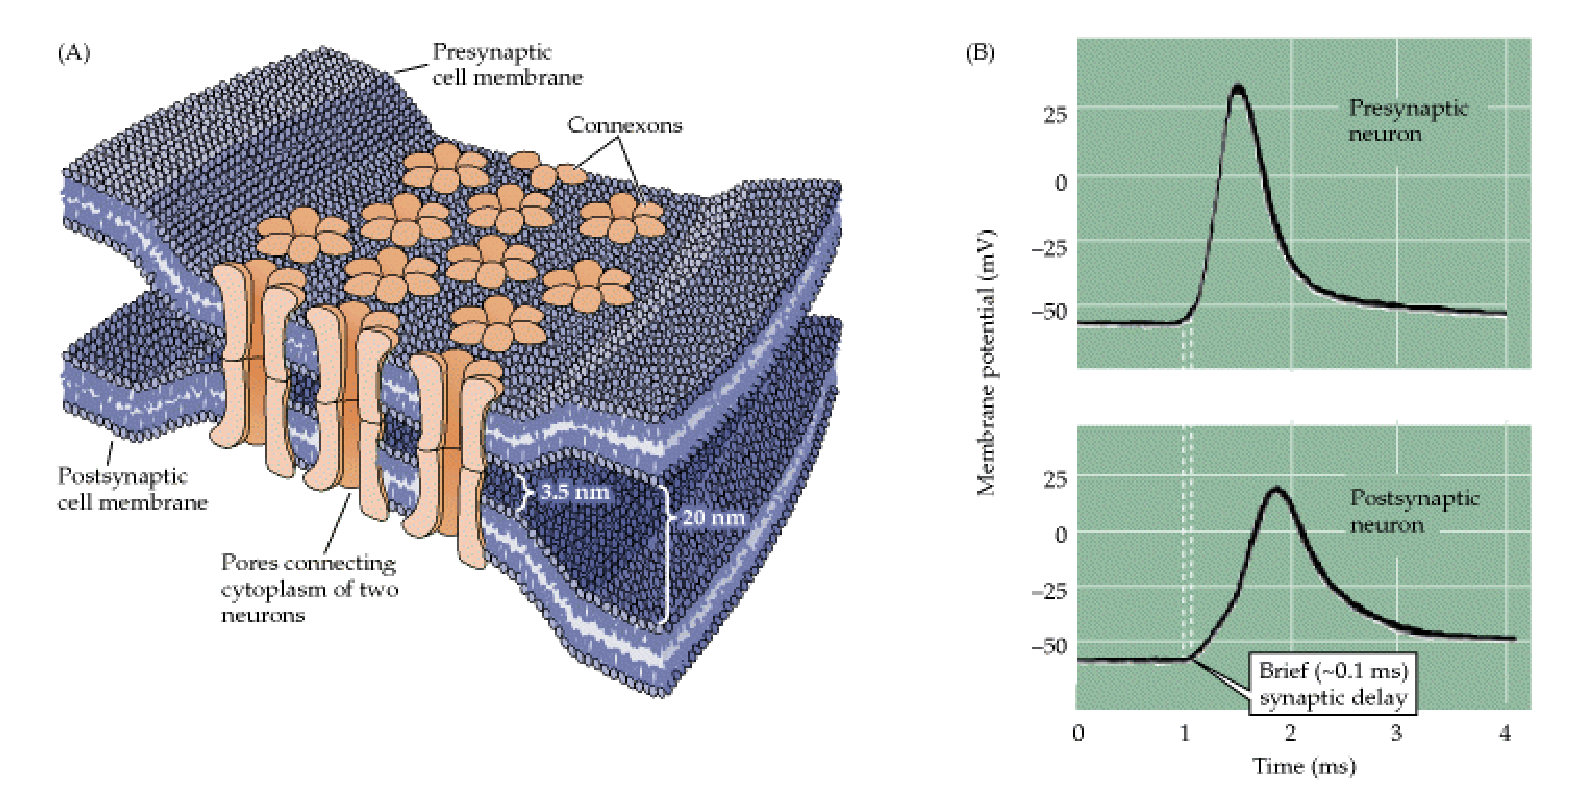
\includegraphics[height=6cm]{./images/gap_junction.eps}}
\caption{Gap junction (a hexameric complex formed by 6 subunits called
connexons which are present in both pre-synaptic and post-synaptic}\label{fig:gap_junction}
\end{figure} 

A key feature is that they provide a simple means of synchronizing the activity
of all interconnected neurons. In adults, these synapses are found in regions of
the brain responsible for certain stereotyped movements, such as jerky movement
of the eyes. Electrical synapses are abundant in non-nervous tissues, such as
cardiac and smooth muscle, where they allow sequential and rhythmic excitation.

%%%%%%%%%%%%%%%%%
\subsection{Chemical synapse: neurotransmitter}
\label{sec:chemical_synapse}

% Signals, in the form of neurotransmitters 
% (Sect.\ref{sec:neurotransmitter}), are transmitted from cells to cells via a
% special gap junction called {\bf synapse} , as shown in Fig.
% \ref{fig:synapse1}. 

A typical chemical synapse (Sect.\ref{sec:synapse}) is made up of two parts: (1)
a knoblike \textcolor{red}{axonal terminal} of the presynaptic neuron, containing many
membrane-bound sacs called {\bf synaptic vesicles} containing {\bf neurotransmitter molecules}.
(2) a \textcolor{red}{receptor region} on the membrane of a dendrite or the cell
body of the postsynaptic neuron, which bears neurotransmitter receptors.
The presynaptic and postsynaptic membranes are separated by the synaptic cleft.
The postsynaptic membrane is on the dendritic spines
(Sect.\ref{sec:dendritic_spines}).

\begin{figure}[htb]
\centerline{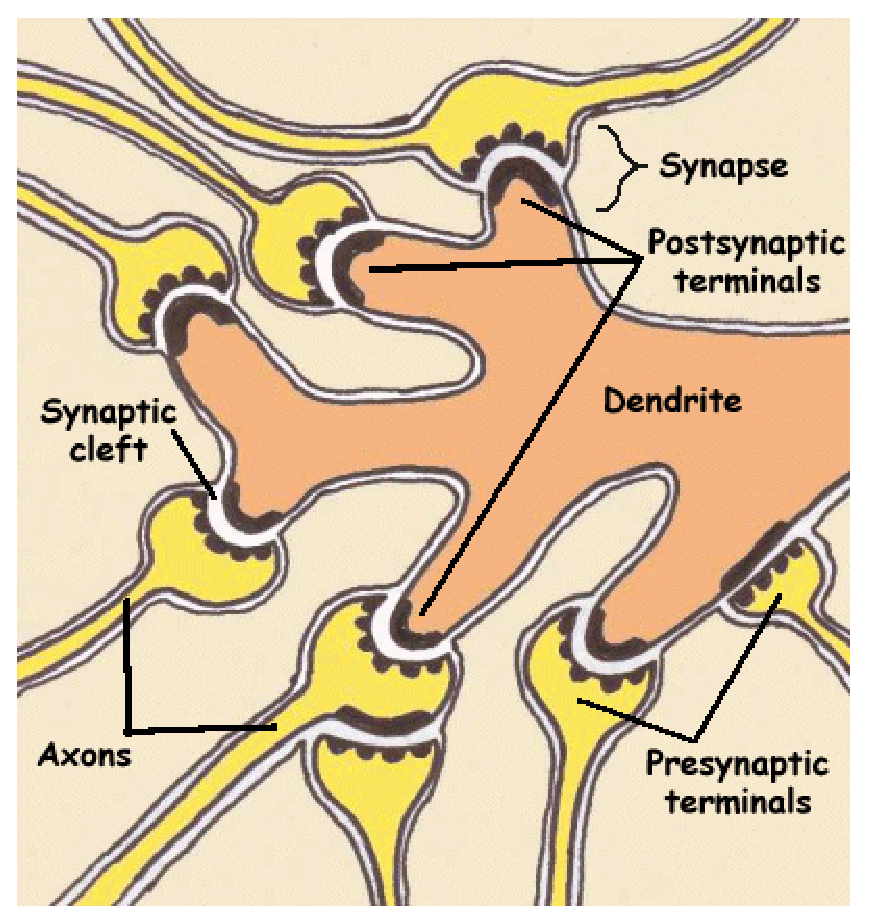
\includegraphics[height=5cm]{./images/synapse.eps}
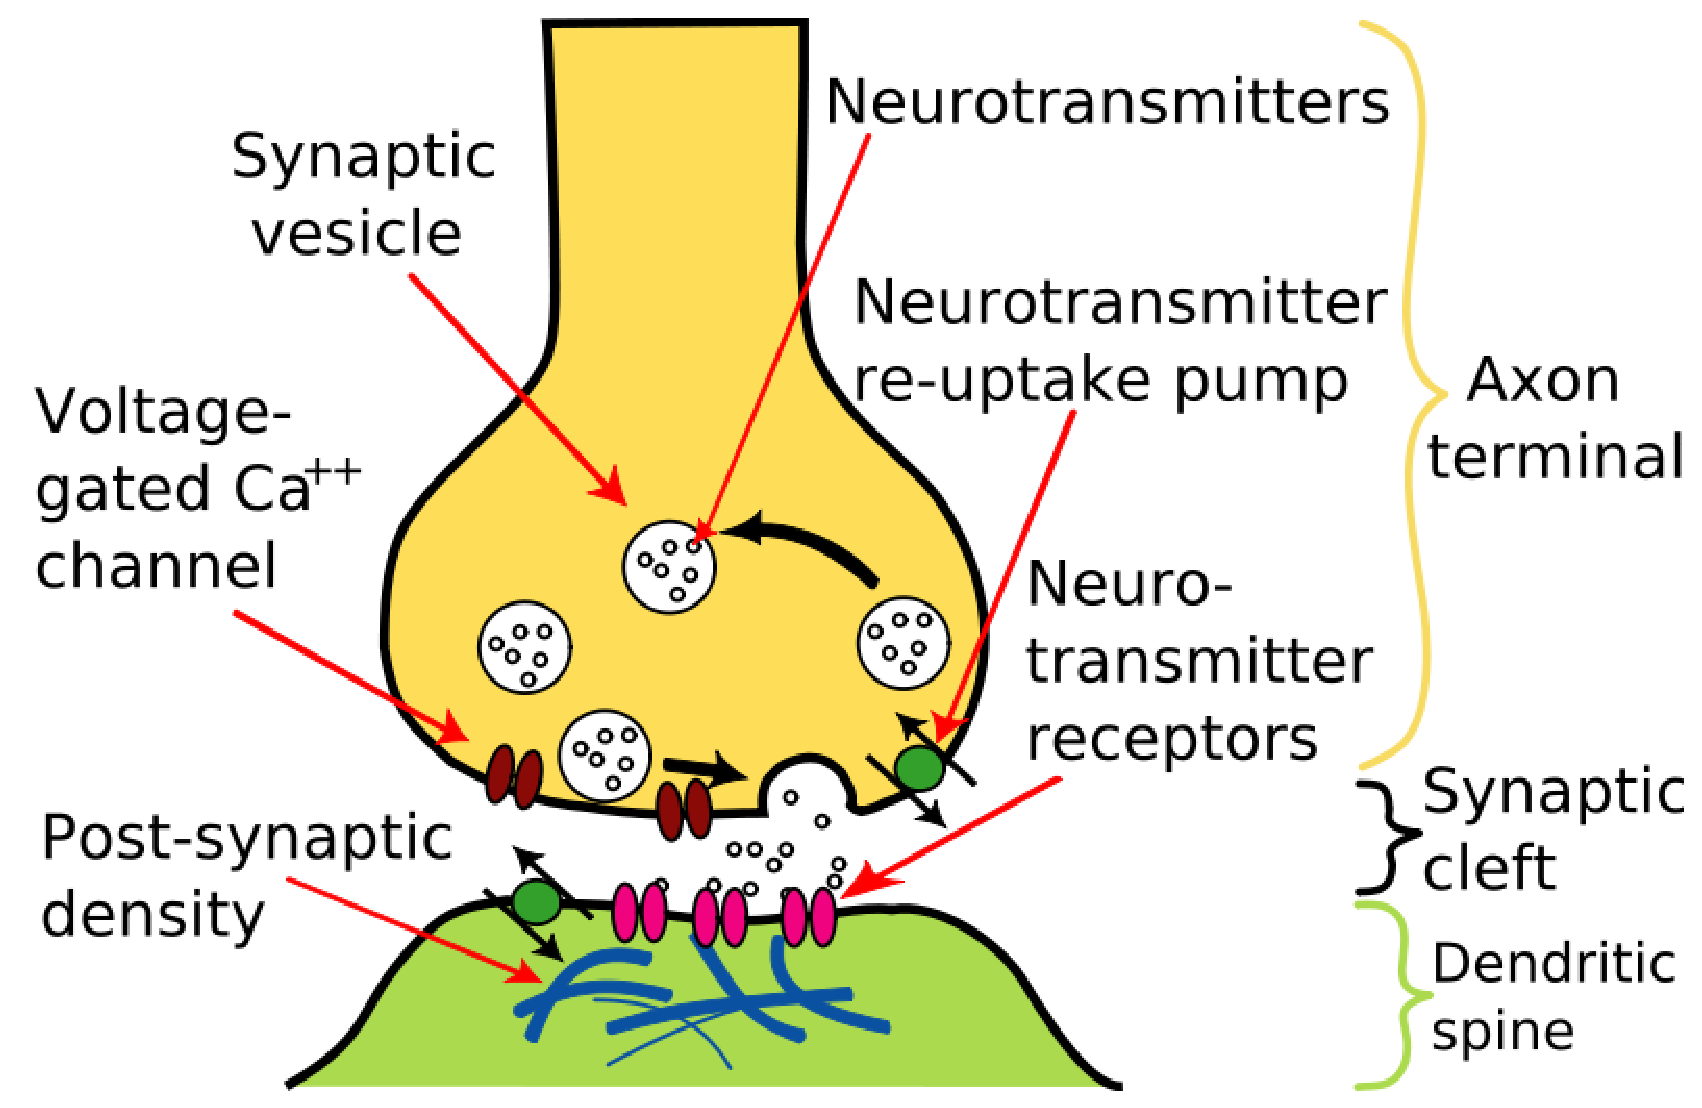
\includegraphics[height=5cm]{./images/synapse1.eps}}
\caption{Chemical synapses}\label{fig:synapse1}
\end{figure} 

The transmission of signals across chemical synapses is a chemical event that
depends on the release, diffusion, and receptor binding of neurotransmitter
molecules and results in unidirectional communication.
At chemical synapse , whenever an electrical signal comes, vesicles from nerve
cell A that contain {\bf neurotransmitters} are released so that the
neurotransmitter can diffuse across the synaptic cleft and bind to the receptors
in the post-synaptic of the next neuron, as shown in Fig.
\ref{fig:synapse}. 


\section{Mechanisms of neurotransmitter releases}
\label{sec:mechanism_neurotransmitter-release}

Bernard Katz pointed out that calcium trigger neurotransmitter release within a
few hundred microseconds, exhibits amazing plasticity and displays a nonlinear
dependence on calcium. Once the AP reaches the axonal terminal, it triggers
$V_m$-dependent $\Ca$ channels, allowing an influx of $\Ca$ ion to do the job.
The question that has been a critical research question was ``how $\Ca$ trigger synaptic vesicle fusion?
how the synaptic vesicle and plasma membrane fuse during neurotransmitter
release (what other proteins involved)''.

They started with identifying all proteins in the presynaptic terminal for
functional studies: synaptophysin, synaptobrevin, synapsins, synaptotagmins,
Munc13s, Munc18s, complexins, RIMs, RIM-BPs, neurexins and neuroligins.
In a review by \citep{sudhof2013}:
\begin{itemize}
  \item The mechanism for membrane fusion known nowadays is the interaction of {\bf
SNAREs} (soluble N-ethylmaleimide-sensitive factor (NSF)-attachment protein
receptors) and {\bf SM proteins} (Sec1/Munc18-like proteins).

  \item The mechanism for $\Ca$ triggered fusion is the binding of $\Ca$ to
{\bf synaptotagmins}, plus a general mechanism of vesicle
positioning adjacent to calcium channels, which involves the interaction of the
so-called {\bf RIM proteins} with these channels and synaptic vesicles.
\end{itemize}

Calcium-binding synaptotagmins act as Ca2+ sensors and involve in
\begin{itemize}
  \item early synaptic vesicle {\it docking} to the presynaptic terminal
  membrane via interaction with $\beta$-neurexin and SNAP-25
  
  \item late steps of synaptic vesicle {\it fusion} to the presynaptic terminal
  membrane
\end{itemize}
\url{http://en.wikipedia.org/wiki/Synaptotagmin_1}

\section{Coincidence detectors}
\label{sec:coincidence-detectors}
%\subsection{Coincidence detectors}

{\bf Coincidence detectors} is the concept in neurobiology meaning that these
molecules (enzyme, protein) are only activated by different signals {\bf
occuring together}.
\footnote{\url{https://en.wikipedia.org/wiki/Coincidence_detection_in_neurobiology}}
Coincidence detection of two distinct signaling events is important for various
aspects of neuronal function (Konnerth et al., 1996).

So, any channels that requires two agents for opening can be a potential 
candidate for coincidence detectors. This is the suspected underlying cellular
mechanisms for STDP (Sect.\ref{sec:STDP}).
However, as there are two types of STDP: LTP and LTD. The question is do they
use the same coincidence detectors?


Here are the popular coincidence detectors:

\begin{enumerate}
  \item NMDAR: detect the coincidence of glutamate release (from presynaptic
  side) and the membrane depolarization (by bAP from postsynaptic side)
  for NMDAR to open.
  
  NMDAR activation is the pre-requisite for the induction of LTP.
  
  \item IP3R: detect the coincidence of IP3 release (IP3 production from
  postsynaptic side) and $\Ca$ elevation for its activation (from postsynaptic
  activity). 
  
  However, IP3R has a biphasic dependency on $[\Ca]$
  (Sect.\ref{sec:IP3R-regulatory-factors}).
  
  \item PLC$\beta$: detect the coincidence of glutamate release (from
  presynaptic side - via activation of mGluR group I or M1/M3 muscarinic
  receptors - Sect.\ref{sec:muscarinic-acetylcholine-receptor}) 
  via its activation and postsynaptic $[\Ca]$ elevation via its catalytic
  function to be performed (i.e. release endocannabinoid).
  
  \citep{hashimotodani2005} confirmed it's PLC$\beta$1 (the major form in
  hippocampus) in hippocampus, with sharply dependency of $[\Ca]$ in the
  physiological range.
  
\end{enumerate}



\section{G protein-mediated signaling pathways}
\label{sec:G_protein_mediated-signaling-pathways}

The G protein-mediated signaling system is a relatively complex signalling
cascade consisting of a family of GTPases receptor - a heterotrimeric G protein
- and an effector. Each component, the receptor, the G protein as well as the
effector can be regulated independently by additional proteins, soluble
mediators, or on the transcriptional level \citep{Wettschureck2005}.


G protein-mediated signaling system has made it by far the most often
employed transmembrane signaling mechanism. 
\begin{itemize}
  \item Sect.\ref{sec:G-protein-coupled-receptor} discuss the different types
  of G protein-coupled receptors

  \item Sect.\ref{sec:GPCR_ligands} discusses the different ligands that can
  bind to each type of G protein-coupled receptor.
  
  \item Sect.\ref{sec:G-protein} discusses the different heterotrimeric G
  protein associated with each G protein-coupled receptor.
  The three main types to be covered are: Gi/o, Gs, Gq/11, and G12/13.
   
%   areleased upon ligand
%   binding on the receptor
    
   Upon the proper type of ligand binding to a given GPCR, the associated G
   protein are activated (Sect.\ref{sec:G-proteins_activation-inactivation})
   
  \item Depending on the type of G protein (or depending on the types of
  stimulus molecules), they may trigger different signaling pathways.

  Here we focus on two signaling pathways:  
  Sect.\ref{sec:phosphatidylinositol-signal-pathway}, 
  and Sect.\ref{sec:cAMP-dependent_pathway}.
\end{itemize}

\subsection{phosphatidylinositol signal pathway: GPCR-PLC-IP3-DAG}
\label{sec:phosphatidylinositol-signal-pathway}
\label{sec:GPCR-PLC-IP3-DAG-pathway}

The pathway is known to form a cornerstone of an ubiquitous transduction
mechanism known to regulate
\begin{enumerate}
  \item metabolism
  \item secretion
  \item contraction 
  \item neural activity
  \item cell proliferation
\end{enumerate}

In the {\it phosphatidylinositol signal pathway}, the activation of G-protein
coupled receptor (GPCR) - Sect.\ref{sec:GPCR}

\begin{verbatim}
Hormone or Neurotransmitters (extracellular) --[bind GPCR]--> 
            change GPCR conformation 
[NOTE: This GPCR associates GDP-Gprotein(alpha,beta)] --[exchange]--> GTP-Gprotein
            --> release GTP-Gq/11 (intracellular)

GTP-Gq/11 --[bind & phosphorylate]--> the nearby membrane-enzyme PLC-beta

==================================================
activated PLC-beta --[cleave PIP2]-->

PIP2  --[hydrolyzed by PLC-beta]-> DAG + IP3
         require Ca2+  
   
   DAG: remain bound to membrane (of glycerol + two fatty acids)
   IP3: diffuse to the inner cell (cytoplasm and bind to IP3R on ER)
   
IP3   --[phosphorylate]--> some proteins
   IP3  [activate IP3R] --> release Ca2+    

DAG   --[activate and change PKC conformation]--> PKC
   released Ca2+ above binds to conventional PKC, trigger its translocation 
   to the membrane where PKC can interact with DAG via C1-domain
   
   activated PKC --[phosphorylate]--> its substrates (some proteins)
   
\end{verbatim}  

As the activation of PLC-beta is 
\begin{verbatim}
PLC-beta --[GTP-Galpha & DAG-sensitive]--> activated PLC-beta
\end{verbatim}

NOTE:
\begin{enumerate}
  \item  $G_{\alpha q/11}$-GTP
(Sect.\ref{sec:Gq/11-protein}) interact with and activate PLC-$\beta$
(Sect.\ref{sec:PLC-beta}) locating on the plasma membrane\footnote{PLC-$\beta$
is an enzyme that cleaves phospholipid  group just before the phosphate
group}~\citep{smrcka1991ip3}.

G$_{\alpha,q/11}$ subunit is activated: can be done at different GPCR
  due to different agonists (alpha1 $\alpha_1$ adrenergic agonists,
  acetylcholine, angiotensin, and vasopressin)
  

  \item PLC-beta - Sect.\ref{sec:PLC-beta}
  
Activated PLC-$\beta$ (which is membrane-bound now) then slides down to cleave a
membrane-bound {\bf PIP2} (Sect.\ref{sec:PIP2}). 

The cleaved PIP2 is hydrolyzed to produce at least 2 second messengers - DAG
(Sect.\ref{sec:DAG}) and IP3 (Sect.\ref{sec:IP3}).

\begin{itemize}

  \item IP3 bind to and open IP3R (Sect.\ref{sec:IP3R}), releasing $\Ca$ from
  the ER store

  \item DAG helps to activate PKC - Sect.\ref{sec:PKC-activation}  
\end{itemize}
    
\end{enumerate}


\subsection{cAMP-dependent pathway}
\label{sec:cAMP-dependent_pathway}


{\bf cAMP-dependent pathway} (adenylyl cyclase pathway) is a signalling pathway
start with GPCR activation (Sect.\ref{sec:G-protein-coupled-receptor}) that
leading to the production of cAMP.
\begin{verbatim}
GPCR --[extracellular-ligand-binding] --> GPCR activation -->
       Gs(alpha)-GDP + GTP -[exchange]-> Gs(alpha)-GTP (activated Gprotein) + GDP 
                                         and then release Gbeta-gamma subunit
       
       Gs(alpha)-GTP -[bind AC] --> Gs(alpha)-GTP-AC
        
       ATP --[Gs(alpha)-GTP-AC]---> cAMP + pyrophosphate 
\end{verbatim}
Adenylyl cyclase is given in Sect.\ref{sec:AC_adenylyl_cyclase}. Degradation of
cAMP is controlled by PDE (Sect.\ref{sec:PDE}).


Upon the increase in cAMP concentration (Sect.\ref{sec:D1R}), cAMP 
leads to
\begin{itemize}
  
  \item activation of cAMP-dependent protein kinase (PKA) enzyme (Sect.\ref{sec:PKA}):  
  
  \item cAMP-regulated guanine nucleotide exchange factors (cAMP-GEFs) -
  Sect.\ref{sec:cAMP-GEF}

  \item PDEs (Sect.\ref{sec:PDE}) (even though PDEs in turns control the
  degradation of cAMP/cGMP)

  \item Popdc (popeye domain containing proteins)

  \item EPAC (exchange proteins activated by cAMP) such as RAPGEF3

  \item enhanced activation of cyclic nucleotide-gated ion channels (CNG
  channels): Sect.\ref{sec:HCN-channels}
   
  Allosteric channel activation: cAMP binds preferentially to open channels
  (at COOH terminus) and locks them in an open state.

  Example: If current in SAN: a half-maximal shift is obtained with a cAMP
  concentration of 0.2 $\muM$ (Sect.\ref{sec:If-current}).

\end{itemize}




\subsection{cGMP-dependent pathway}
\label{sec:cGMP-dependent-pathways}

The downstream effector of cGMP (Sect.\ref{sec:cGMP}) is cGMP-dependent protein
kinase (PKG - Sect.\ref{sec:PKG}), cyclic nucleotide-gated ion channels, and
PDEs (Sect.\ref{sec:PDE}) (even though PDEs in turns control the degradation of
cAMP/cGMP).

\subsection{Pyrophosphate (PPi)}
\label{sec:pyrophosphate}
\label{sec:PPi}
\label{sec:ANK-channel}

\textcolor{red}{Pyrophosphate} (i.e. $\ce{P2O7^{4-}}$ or abbreviated as PP$_i$)
is an anion; formed by the hydrolysis of ATP and AMP (e.g. cAMP, cGMP) -


\begin{verbatim}
ATP -----[AC]------>  cAMP + (PO4-PO3)^{4-}
\end{verbatim}

Cells may channel intracellular PPi into extracellular fluid (ECF)
\begin{itemize}
  \item   ANK is a nonenzymatic plasma-membrane PPi channel that supports
  (bringing up) extracellular PPi levels.
  
  Defective function of the membrane PPi channel ANK is associated with low
  extracellular PPi and elevated intracellular PPi
  
  \item  Ectonucleotide pyrophosphatase/phosphodiesterase (ENPP) may function to
  raise extracellular PPi
    
\end{itemize}

\subsection{Gbetagamma-mediated signaling pathway}
\label{sec:Gbetagamma-mediate-signaling-pathway}

The G$\beta\gamma$ complex include different forms of $\beta$ subunit
($\beta$1-5) and $\gamma$ subunit ($\gamma$1-12), which then can perform
different signalling function

\begin{itemize}
  \item increase/reduce AC
  
  \item increase PLC
  
  Example: PLC-beta (Sect.\ref{sec:PLC-beta})
  
  \item increase PI3K
  
  \item increase PKC
  
  \item increase PKD
  
  \item increase GPCR kinase activity
  
  \item modulate $\Ca$ and $\K$ channels
\end{itemize}
\url{http://lsresearch.thomsonreuters.com/maps/641/}


\subsection{Cross-talk between GPCR}

\textcolor{red}{Control intracellular $[\Ca]$}:
It has been well documented that Ca(2+) signalling by one type of GPCR can be
influenced by stimulation of a different type of GPCR.
So, it may be critical to improve the cell function on the understanding of the
positive-feedback or negative-feedback regulation and the likely shared
components of the above different signalling pathways.

There is currently no single mechanism that adequately accounts for all examples
of this type of cross-talk. Indeed, many studies either have not addressed this
issue or have been unable to determine the mechanism(s) involved
(review: \citep{werry2003}).


\section{Synaptic potential (Postsynaptic potential)}
\label{sec:postsynaptic_potential}
\label{sec:synaptic_potential}

Synaptic potential (or postsynaptic potential) refers to the difference in
voltage between the inside and outside of a postsynaptic neuron. In other words,
they are the ``incoming" signal of a neuron. \textcolor{red}{Synaptic potential
comes in two forms: excitatory
(Sect.\ref{sec:excitatory_postsynaptic_potential}) and inhibitory
(Sect.\ref{sec:IPSP}).}


\begin{figure}[htb]
  \centerline{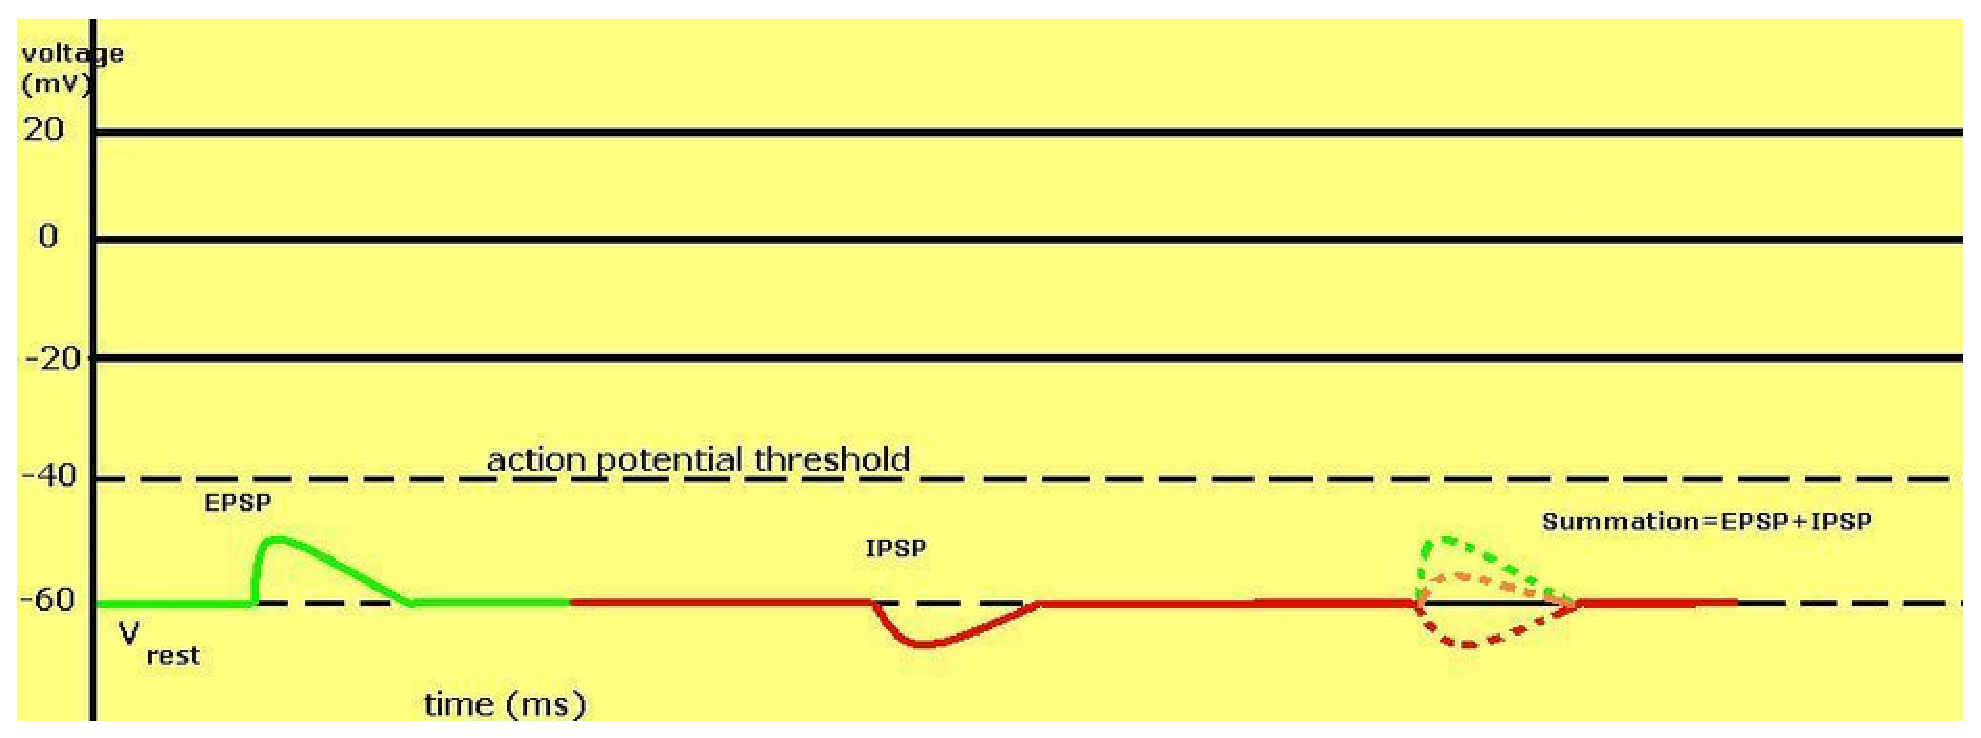
\includegraphics[height=5cm]{./images/EPSP_IPSP.eps}}
\caption{EPSP and IPSP}
\label{fig:EPSP_IPSP}
\end{figure} 

\section{Postsynaptic current}
\label{sec:postsynaptic-current}



\subsection{EPSC}
\label{sec:EPSC}

The flow of ions that causes an EPSP (Sect.\ref{sec:EPSP}) is an excitatory
postsynaptic current (EPSC). 

{\bf Excitatory postsynaptic current} (EPSC) is any postsynaptic current which
depolarize the postsynaptic membrane potential (e.g. caused by inward $\Ca$
current) which increases the likelihood of generating a somal action potential
(Sect.\ref{sec:AP-neuron-soma}), Fig.\ref{fig:EPSC_IPSC}(A).

\begin{figure}[hbt]
  \centerline{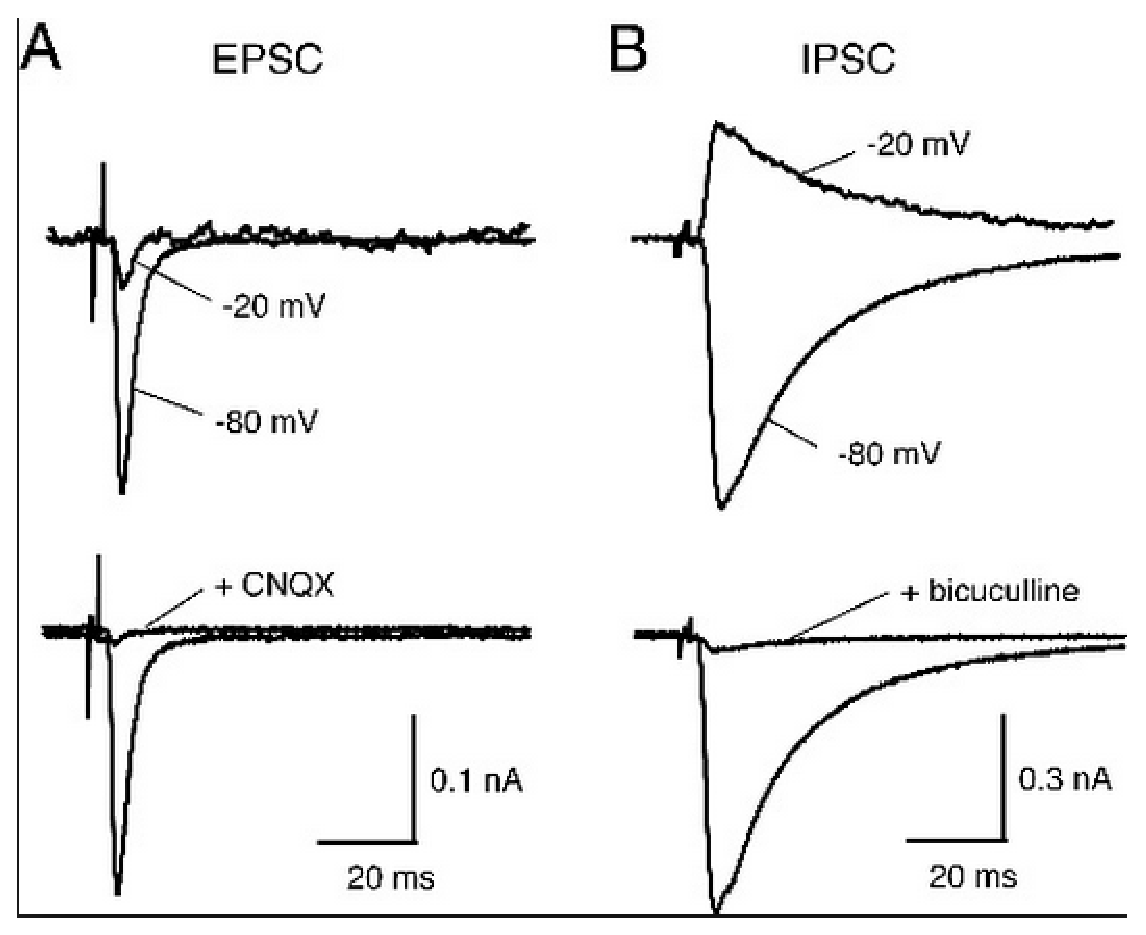
\includegraphics[height=4cm,
    angle=0]{./images/EPSC_IPSC.eps}}
\caption{(A) EPSC. (B) IPSC}
\label{fig:EPSC_IPSC}
%http://mhs3.mp.kanazawa-u.ac.jp/eng/staff/rihabiri/shosaku.html
\end{figure}

EPSC is often experimentally recorded as the mean amplitudes were the average of
a number (e.g. 25) of evoked EPSCs.
EPSCs amplitude is proportional to $npq$, with 
\begin{enumerate}
  \item  $n$ being the number of releasing sites, 
  
  \item $p$ the probability of release,
  and 
  
  \item $q$ the quantum size (unit: mV). 
\end{enumerate}
It is admitted that $n$ and $p$ describe presynaptic events, and $q$
is the postsynaptic indicator.

To test which factors play a role in changing EPSC, 
it is deduced from the relationship between normalized CV$^{-2}$ and normalized
EPSC.
\begin{itemize}
  \item If normalized CV$^{-2}$ > normalized EPSC amplitude: both $n$ and $p$
  can vary
  
  \item If normalized CV$^{-2}$ = normalized EPSC amplitude: only $n$ can vary
  
  \item If normalized CV$^{-2}$ < normalized EPSC amplitude: changes in EPSC
  amplitude are related to variation in $n$, $p$, and $q$ (indicating a mixed
  of presynaptic and postsynaptic origin of modifications).
  
  \item A variation of normalized EPSC amplitude
without any variation of normalized CV$^{-2}$: only $q$ can vary (i.e.
postsynaptic modifications)
\end{itemize}

\begin{enumerate}
  \item The normalized CV$^{-2}$ is
\begin{equation}
\text{normalized CV}^{-2} = \frac{\text{CV}^{-2}\text{ after induction of
plasticity}}{\text{CV}^{-2}\text{ control}}
\end{equation}
with CV$^{-2}$ is used, and
CV is the EPSC's coefficient of variations (calculated as the ratio of SD and
the mean of EPSC amplitude).

  \item The normalized EPSC amplitudes
\begin{equation}
\text{normalized EPSC} = \frac{\text{EPSC mean amplitude after induction of
plasticity}}{\text{control EPSC mean amplitude}}
\end{equation}
\end{enumerate} 

In Fino et al. (2005) experiment, the success rate for a cortical stimulation
leading to a recorded EPSC on D2+ MSN is almost 100\%. The data also suggested a
monosynaptic corticostriatal transmission, i.e. only one synapce is activated.
The electrical stimulus to cerebral cortex was adjusted in order to evoke
striatal excitatory postsynaptic currents (EPSCs) ranging from 50 to 200 pA
amplitudes.

\subsection{-- Spontaneous sE(I)PSCs}

Both sE(I)PSC and mE(I)PSCs are similar in the fact that they occur without any
artificial stimulation.
The difference between sE(I)PSCs and mE(I)PSCs is coming from the fact that in
case of the sE(I)PSCs there is a chance of action potential-driven events due to
intrinsic properties of presynaptic cell and/or network activity.



\subsection{-- Miniature EPSC (mEPSC)}
\label{sec:mEPSC}

\begin{mdframed}

Miniature synaptic potentials was first used at the frog neuromuscular junction,
Fatt and Katz (1952) referred to them as 'miniature spontaneous end plate
potentials, and the subsequent terminologies "spontaneous epsps" or "miniature
epsps" are often used interchangeably. However, there are some distinctions (see
below).

% Fatt, P. and Katz, B. 1952. Spontaneous subthreshold activity at motor nerve-endings.
% J. Physiol. 117:109-128.

Under some physiological conditions, such as in saline solution with a low
concentration of calcium ions, evoked EPSP are reduced in amplitude and
waveform to the same values as the spontaneous miniature epsps, hence while
under those conditions the two events resemble one another in both amplitude and
time course, they are technically different.

\textcolor{red}{The frequency of the mPSC is dependent upon vesicular release
whereas the amplitude of the mPSC is dependent upon activation of the
postsynaptic receptor.} E.g.: if you see a reduction in the frequency of mIPSCs,
it is due to a decrease in the release of GABA, while a decrease in the
amplitude of mIPSCs is due to reduced activation of postsynaptic GABAA
receptors. 

Another hypothesis (the reduction mPSC is caused by the change in presynaptic
side, i.e. reduced quantal size since the uptake of choline was impaired): A
drug referred to as hemicholinium interferes with the re-uptake of choline at
the vertebrate neuromuscular junction; prolonged exposure to hemicholinium leads
to a gradual reduction in the amplitude of the miniature end plate potentials,
even though the site of action is at the (presynaptic) motor terminals (Elmquist
et al., 1963).

However, this can also be explained by the post-synaptic side affect, i.e. an
accumulation of ACh at cholinergic synapses often leads to desensitization of
the receptors.

% Elmquist, D., Quastel, J.M., Thesleff, S. 1963. Prejunctional action of HC-3 on
% neuromuscular transmission. J.Physiol. 167:47-48 P. 

\url{https://www.researchgate.net/post/What_is_the_exact_difference_between_spontaneous_sEPSP_Cs_and_sIPSP_Cs_and_mini_mEPSP_Cs_and_mIPSP_Cs_postsynaptic_potentials_or_currents}
\end{mdframed}


Both sE(I)PSC and mE(I)PSCs are similar in the fact that they occur without any
artificial stimulation.
In case of the sE(I)PSCs there is a chance of action potential-driven events due
to intrinsic properties of presynaptic cell and/or network activity

All the mE(I)PSCs, in turn, are recorded in the presence of tetrodotoxin (TTX)
which blocks action potential formation (from both presynaptic neurons and
postsynaptic neurons) and its propogation, thus mE(I)PSCs are more "spontaneous"
events than sE(I)PSCs, i.e. mE(I)PSC is thought to correspond to the response
that is elicited by a single vesicle of transmitter.
Thus, mE(I)PSC can be further used for the quantification of readily releasable
pool size.

Having both sE(I)PSCs and mE(I)PSCs can help to understand where the changes in
synaptic trasmission are coming from. Whether it is from the presynaptic side,
or postsynaptic or both. Thus, it is useful to take both  sE(I)PSCs and
mE(I)PSCs  from the same cell.
First, one can record the sE(I)PSCs and then, by introducing TTX into bath
solution the mE(I)PSCs.

\textcolor{red}{\bf Triggering protocol}
\begin{enumerate}
  \item  Miniature excitatory synaptic current (mEPSC) is typically recorded in the
presence of TTX (0.5$\muM$), i.e. to block Na current.
  
  \item Glutmate (0.5 mM) is uncaged (brief 5ms pulse of glutamate is applied
  through pipette) into the extracellular environment, which may activates
  multiple synapses (Segal et al., 2003)
  
  \item 
\end{enumerate}

\textcolor{red}{\bf Recorded signal}
\begin{itemize}
  \item the change in fluorescence which is mapped to the current generated
  
  \item recorded at neuronal somata near pipette tip (where glutamate is
  released)
\end{itemize}


The weighted mean single channel conductance was 20.4 pS, suggesting that a
single quantum opens 22 postsynaptic glutamate receptor channels on average.
Given the estimated number of AMPAR near the site is about 400, not all of them
are actually activated.



\begin{enumerate}
  \item  AMPA receptor-mediated miniature EPSC: the fast component
  
  \item NMDAR-mediated mEPSC: the slower component
  
  \item AMPAR + NMDAR-mediated mEPSC: has both fast and slow component
\end{enumerate}


\begin{enumerate}
  
  \item in orexin neurons (Sect.\ref{sec:orexin-neuron}): AMPAR-mediated mEPSCs
  showed heterogeneous time course:  some mEPSCs had fast rise and decay (fast
  mEPSC), while some had longer kinetics, smaller amplitude but larger
  integrated area (slow mEPSC).
  
  The dopamine agonists altered the frequency as previously reported, but had no
  effect on the rise, decay or area of mEPSC, suggesting that dopamine affects
  fast and slow mEPSCs equally.
  
  This suggested distinct subset of excitatory synaptic inputs are processed
  differently by orexin neurons .
  
  \item in mossy fiber-granule cell synapse:
  Sect.\ref{sec:mEPSC-mossy-fiber-granule-cell}
  
  
  \item in striatal neuron (2-3 week culture from prenatal striatal neuron):
  Vrest = -60mV; high Rin = 540$\pm$ 110 M$\Omega$:
  
  No spontaneous excitatory synaptic current was found; yet occasionally express
  inhibitory postsynaptic current.
  
  
  
\end{enumerate}

\subsection{-- Evoked EPSC (eEPSC)}
\label{sec:eEPSC}

Evoked EPSC are EPSC generated by action potential from the presynaptic neurons
(e.g. presynaptic neuron is triggered by brief (1 ms) depolarizing pulses.);
which may activate many synapses. So, eEPSC typically is larger.

It's just that the arrival of pre-synaptic action potentials at the synapse
raises the probability of quantal release.

\begin{enumerate}
  
  \item record evoked AMPAR current from
  culture rat hippocampal neurons.
  
  \item record evoked AMPAR + NMDAR current from culture rat hippocampal
  neurons.
  
\end{enumerate}

\subsection{IPSC}
\label{sec:IPSC}

{\bf Inhibitory postsynaptic current} (IPSC) is any postsynaptic current which
hyperpolarizes the postsynaptic membrane potential (e.g. inward $\Cl$ current),
i.e. reduces the likelihood of an asomal action potential,
Fig.\ref{fig:EPSC_IPSC}(B).
Typically this is mediated by an increase in chloride conductance  (inward) or
potassium conductance (outward). Inhibitory postsynaptic current is usually
synonymous with an evoked inhibitory post synaptic current.


\section{Excitatory Postsynaptic potential (EPP, EPSP)}
\label{sec:excitatory_postsynaptic_potential}

There are two terms to refer to excitatory postsynaptic potential: {\bf EPSP}
(when linking between 2 neurons - Sect.\ref{sec:EPSP}) and {\bf EPP} (when
linking between a muscle cell and a neuron - Sect.\ref{sec:EPP}) (see discussion
below). The reason to discriminate as there are two fundamental differences
between the process of synaptic transmission at the sensorimotor synapse in the
spinal cord and the process of synaptic transmission at the neuromuscular
junction.
\begin{itemize}
  \item transmitter substance released by the sensory neuron is amino acid
  glutamate (Sect.\ref{sec:glutamate_receptor}), not ACh.
  
There are more than 50 different neurotransmitters, but they can be groupped
into 4 basic categories (Sect.\ref{sec:neurotransmitter}).

  \item The amplitude of the postsynaptic potential in spinal motor neuron, as a
  result of an action potential in a 1A afferent fiber, is only about 1 mV;
  while the amplitude of that in neuromuscular junction is 50 mV.
  
QUESTION: \textcolor{red}{How 1-mV EPSP can trigger the AP in motor neuron}?
This is explained by the multiple action potentials in many different stretch
receptors under the stretch of the muscle fibers.
In fact, the greater the stretch, the greater is the probability of activating
more stretch receptors. This process is referred to as recruitment, which can
comes from multiple fires from a single neuron (temporal summation) or multiple
neurons (spatial summation).
% The processes by which the multiple EPSPs from presynaptic neurons summate over
% space and time are called temporal and spatial summation. 
\end{itemize}

The release of neurotransmitter vesicles from the presynaptic cell is
probabilistic. In fact, even without stimulation of the presynaptic cell, a
single vesicle will occasionally be released into the synapse, generating
{\bf miniature EPSPs} (mEPSPs). The mEPSP at the neuromuscular junction is
called {\bf miniature EPP} (mEPP). The study was pioneered by
Bernard Katz in 1951.

The quantal nature of this stochastic release can be defined by 2 terms
\begin{itemize}
  \item {\it quantal size}: the synaptic response to the release of
  neurotransmitters from a single vesicle

NOTE: With stochastic release of acetylcholine (ACh) from a single vesicle, mEPP
is about 0.5 mV, the smallest possible depolarization which can be induced in a
muscle. \url{http://en.wikipedia.org/wiki/End-plate_potential}
  
  \item {\it quantal content}: the number of effective vesicles released in
  response to a nerve impulse
\end{itemize}
{\it Quantal analysis} refers to the methods used to deduce, for a particular
synapse, how many quanta of transmitter are released and what the average effect of each
quantum is on the target cell, measured in terms of amount of ions flowing
(charge) or change in the membrane potential.


\subsection{EPSP: Glutamate receptors}
\label{sec:EPSP_mechanism}
\label{sec:EPSP}

{\bf Excitatory Post-Synaptic Potentials} (EPSP): is a postsynaptic potential,
i.e. membrane depolarization at the synaptic site which then propagate to the
soma and help depolarizing the somatic membrane potential in that making the
neuron more likely to fire an AP, Fig.\ref{fig:EPSP_IPSP}.

EPSPs is the result of inward currents (at postsynaptic side), or can also
result from a decrease in outgoing positive charges, while IPSPs are sometimes
caused by an increase in positive charge outflow.

It can take place at the excitatory {\it chemical synapse}
(Sect.\ref{sec:synapse})
\begin{itemize}
  \item ACh (Sect.\ref{sec:Acetylcholine}
  
  \item Glutamate (Sect.\ref{sec:Glutamate}):

It has been reported that NMDAR contributes to only 16\% of the amplitude of
excitatory postsynaptic potential (EPSP) in pyramidal cells of cortical layer
2/3, compared with 39\% of EPSP amplitude in spiny neurons of layer 4.
A similar observation is obtained by \citep{wang2006}: using AMPAR antagonist -
CNQX - it reduces LFP signals in response to whisker stimulation by an average
of 69.1$\pm$ 4.0; while NMDAR antagonist - D(-)-amino-7-phosphonovaleric acid
(AP5) delivered by ionotophoresis - does not alter LFP signal.

\end{itemize} 
%with the neurotransmitter is ACh (Sect.\ref{sec:Acetylcholine}.
This small depolarization is a result of the flow of positively charged ions into
the postsynaptic cell.  The net flow of ions that causes an EPSP is an
excitatory postsynaptic current (EPSC).

  
\textcolor{red}{EPSPs, like IPSPs, are graded, not an all-or-none beahvior}.
Larger EPSPs result in greater membrane depolarization and thus increase the
likelihood that the postsynaptic cell reaches the threshold for firing an action potential.

EPSPs and IPSPs compete with each other at numerous synapses of a neuron; this
determines whether or not the action potential at the presynaptic terminal will
regenerate at the postsynaptic membrane.


Fig.\ref{fig:EPSP_summation} shows how multiple EPSPs from different synapses
of the same cell can work to trigger an AP. 

In some areas of the brain, such as the hippocampus, neurons are arranged in
such a way that they all receive synaptic inputs in the same area. Here, EPSP is
not recorded from a single cell, but from a population of neurons, and is calld
a {\bf field potential}, or field EPSP in studying hippocampal long-term
potentiation (LTP) of CA1 region. This is called population spike (PS)
\url{http://en.wikipedia.org/wiki/Population_spike}

\begin{figure}[hbt]
  \centerline{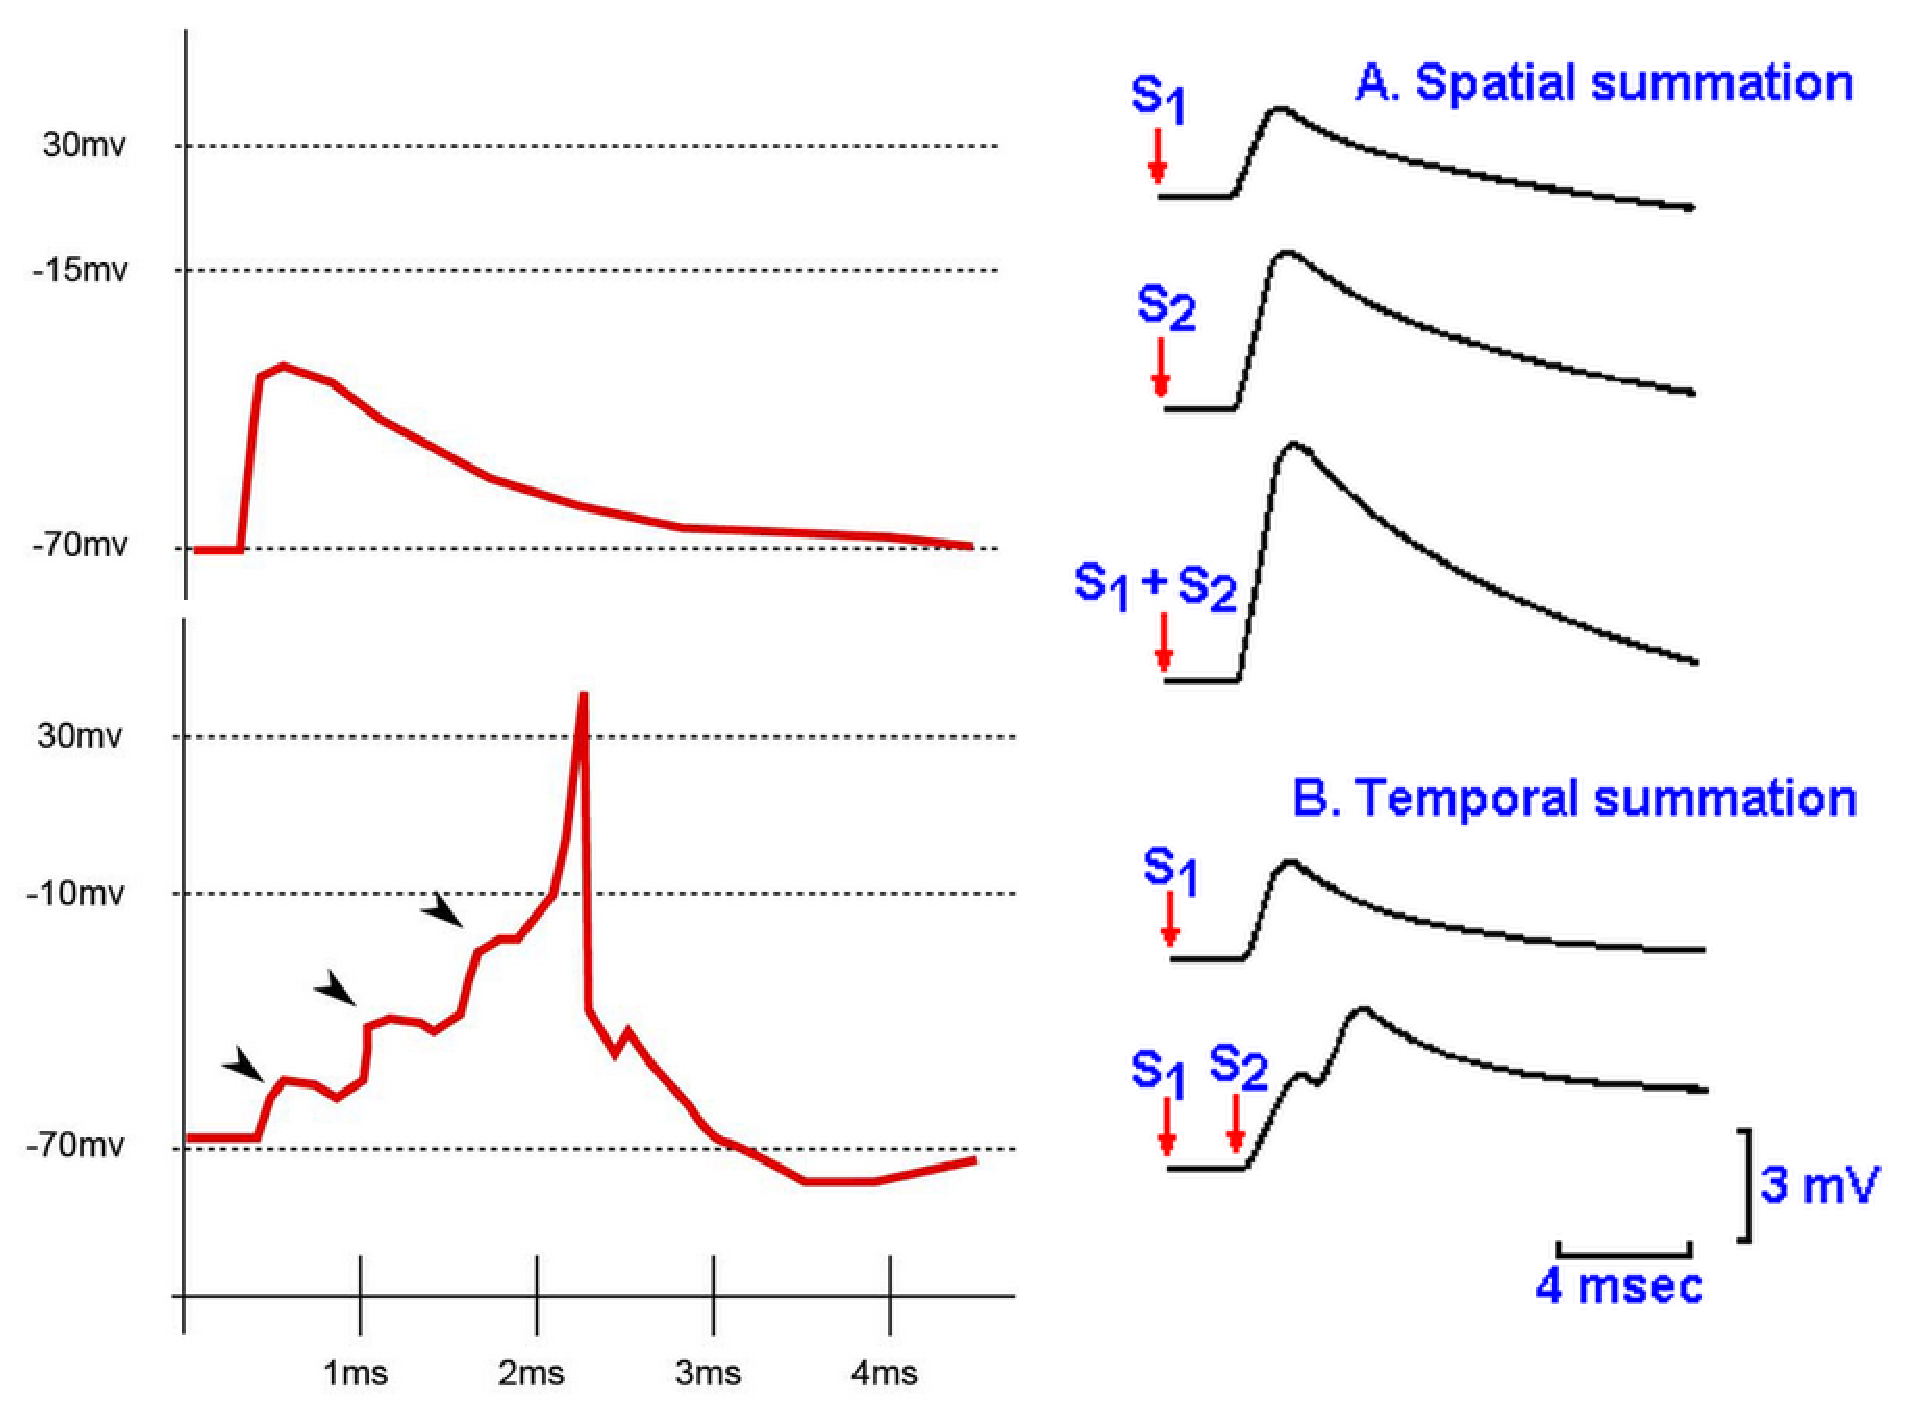
\includegraphics[height=7cm,
    angle=0]{./images/EPSP_summation.eps}}
  \caption{EPSP: temporal summation and/or spatial summation, that can lead to
  a depolarization that can generate an AP}
\label{fig:EPSP_summation}
\end{figure}
\url{http://en.wikipedia.org/wiki/Excitatory_postsynaptic_potential}

EPSPs are amplified by persistent sodium ion conductance in external nerve
cells. Low-voltage activated calcium ion conductance enhances even larger EPSPs.


There are different strategies to model an EPSP:
\begin{enumerate}
  \item as an input current into the dendritic compartment - Sect.\ref{sec:EPSP-model-synaptic-input-Hoffman1997}
  
  \item as a detailed model with a separate compartment for spine head and neck
  with a number of ion channels and receptors on it.
  
  \item ???
\end{enumerate}

\subsection{EPP (skeletal neuromuscular junction): ACh receptor}
\label{sec:EPP_mechanism}
\label{sec:EPP}

{\bf End Plate Potential} (EPP) looks and behave much like EPSP
(Sect.\ref{sec:EPSP}), but it refers to the depolarization at the neuromuscular
junction (i.e. the junction between a nerve cell and a muscle cell). EPP is
mediated by neurotransmitter acetylcholine (ACh).

Once Acetylcholine are released from the presynaptic terminal, it move to and
bind to the receptors on the postsynaptic membrane. All acetylcholine receptors
in the neuromuscular junction are nicotinic.

These receptors are slow and therefore are unable to measure a miniature end
plate potential (mEPP). The acetylcholine vesicles
(Sect.\ref{sec:Acetylcholine}) release their entire quantity of acetylcholine
and this causes miniature end plate potentials (MEPPs) to occur which are less
than 1mV in amplitude and not enough to reach threshold.


\subsection{slow synaptic potentials: metabotropic receptors}

The mechanism of these slow synaptic responses involves changes in metabolism
of the cell. 



\section{Inhibitory Postsynaptic potential}
\label{sec:IPSP}
\label{sec:IPSP_mechanism}

NOTE: {\bf Inhibitory postsynaptic potentials} (IPSPs) is a postsynaptic
hyperpolarized potential (at chemical synapse), Fig.\ref{fig:EPSP_IPSP}, 
as a result of the flow of ions that cause a decrease in membrane
potential, i.e the increased permeability of the membrane to 

\begin{enumerate}
  
  \item  negative ions (e.g. Chloride $\Cl$) into the cell or
  
  \item positive ions ($\K$) out of the cell, or 
  
  
  \item both.
    
\end{enumerate}

The gating of the ion channels for these ion flow as a result of inhibitory
neurontransmitter (e.g. GABA - Sect.\ref{sec:GABA}, and glycine
(Sect.\ref{sec:Glycine})) binding to ???, causing IPSC (Sect.\ref{sec:IPSC}).
 

% In terms of inhibitory postsynaptic potential,
% we have IPSP
% 
% IPSPs always want to keep the membrane potential more negative than the  action
% potential threshold and can be seen as a transient hyperpolarization.

